\section{Circuits for Pauli Maps}
\label{sec: Circuits for Pauli Maps}

\begin{itemize}
\item \textbf{Circuit for a Pauli channel:}  Propose a circuit to simulate a Pauli channel on $n$ qubits. It works by creating a $2n$-qubit state on ancilla qubits.
\item \textbf{Simulation:} Show the fidelities of simulating the circuit on a quantum computer for many one-qubit channels inside the tetrahedron.
\item \textbf{For Pauli dynamical maps}: See how the circuit generalizes to parametrized channels and notice that many rotations are needed to create the $2n$-ancilla qubit state. \\
\end{itemize}

In this section we introduce the concept of Pauli channels and 
Pauli dynamical maps, as well as proposal for a quantum circuit that simulates them on systems of $N$ qubits. 
Furthermore, we show the results of implementing the circuit on a 
quantum computer for the particular case of Pauli channels of one qubit. 

\subsection{Quantum Channels}
\label{subsec: Quantum Channels}
Quantum channels are the most general linear operations that a 
quantum system (which is represented by a density matrix $\rho$) 
can undergo independently of its past~\cite{zimansbook,cirac}. 
These channels are constructed based on three fundamental properties: 
linearity, trace preservation, and complete positivity.

Linearity ensures that a quantum channel $\mathcal{E}$ maps any convex combination 
of density matrices into a convex combination of their evolution. 
The trace preserving property is given by $\tr \mathcal{E}[\rho] = \tr \rho = 1$ 
and guarantees that the quantum channel occurs with a probability of 1. 
The complete positivity condition ensures that the quantum channel preserves positive semidefiniteness. 
A linear map $\mathcal{E}$ is considered positive if it maps density operators to density operators 
($\mathcal{E}(\rho) \geq 0$  for all density matrices $\rho$). 
If the extension of a positive map to include an ancilla results in another positive map, 
the original map is said to be completely positive~\cite{geometry}. 
This property is required for quantum channels to allow for the
proper evolution of potentially entangled states with an ancilla.

Jamiołkowski and Choi~\cite{choi,jamil} developed a simple algorithm to test for 
complete positivity of a quantum channel. 
The algorithm exploits the isomorphism between a channel $\mathcal{E}$ and the 
state $\mathcal{D} = (\text{id} \otimes \mathcal{E}) [|\Omega \rangle \langle  \Omega|]$, 
where $|\Omega\rangle$ is a maximally entangled state between the original system and an 
ancilla and “id” is the identity channel. 
Remarkably, the map $\mathcal{E}$ is completely positive if and 
only if $\mathcal{D}$ (also known as the Choi or dynamical matrix of $\mathcal{E}$) is positive semidefinite.


\subsection{Pauli Channels}
\label{subsec: Pauli Channels}

To define a Pauli channel, we start by exploring the single-qubit scenario and then the $N$-qubit one. 
First of all, the most general single-qubit density matrix can be written as
\begin{equation}
\label{ec: Density Matrix}
\rho = \dfrac{1}{2} \sum_{\alpha=0}^{3} r_{\alpha} \sigma_{\alpha},
\end{equation}
with $\sigma_0 = \mathbb{I}$, and $\sigma_{1,2,3}$ the usual Pauli matrices. 
Normalization requires that $r_0 = 1$ and the remaining $r_{1,2,3}$ form a Bloch vector. 
A Pauli channel is defined as an operation
that applies a convex combination of Pauli matrices to the density matrix in the following way:
\begin{equation}
\label{ec: Pauli channel 1 qbit}
\mathcal{E}(\rho) = \sum_{\gamma=0}^3 k_{\gamma} \sigma_{\gamma} \rho \sigma_{\gamma},
\end{equation}
where $k_{\gamma}$ are non-negative real numbers such that 
$\sum_{\gamma} k_{\gamma} = 1$ (these conditions are needed for the channel 
to be completely positive and trace preserving). 

Having defined the one qubit case, 
in order to present the $N-$qubit one, we 
need to introduce the so-called \textit{Pauli strings}, defined as
\begin{equation}
\label{ec: Density matrix Nqbit}
\sigma_{\vec{\alpha}} = \sigma_{\alpha_1} \otimes \sigma_{\alpha_2}\otimes \cdots \otimes \sigma_{\alpha_N},
\end{equation}
where $\vec{\alpha}$ denotes a multi-index $(\alpha_1, \cdots, \alpha_N)$
 and $\alpha_i \in \{0,1,2,3\}$. 
 These operators form an orthogonal basis in the space of operators acting on $N$ qubits. 
 Similarly to the single-qubit case, the density matrix $\rho$ 
of a system of $N$ qubits can be written using Pauli strings as:
\begin{equation}
\label{ec:cap2-1}
\rho = \dfrac{1}{2^N} \sum_{\vec{\alpha}} r_{\vec{\alpha}} \sigma_{\vec{\alpha}}.
\end{equation}
Then, we define a Pauli channel as a transformation of the density 
matrix given by
\begin{equation}
\label{ec: pauli channel N-qubt}
\mathcal{E}(\rho) = \sum_{\vec{\gamma}} k_{\vec{\gamma}} \sigma_{\vec{\gamma}} \rho \sigma_{\vec{\gamma}},
\end{equation}
where just as before, complete positivity and trace preservation requires
that $k_{\vec{\gamma}}$ are positive real numbers such 
that $\sum_{\vec{\gamma}} k_{\vec{\gamma}}=1$.

\subsection{Circuit for a Pauli Channel}

We are interested in constructing a quantum circuit that can implement an
arbitrary Pauli channel on a system of $N$ qubits. 
To do it, it is important to realize that a Pauli channel
 as shown in equation \ref{ec: pauli channel N-qubt}  can 
be interpreted as as a transformation that applies
each Pauli operator $\sigma_{\vec{\gamma}}$ on $\rho$ with a probability $k_{\vec{\gamma}}$.

Given this interpretation of the channel, 
it is easy to construct a quantum circuit that implements 
it with the help of $2n$ ancilla qubits.
The general idea is to first construct a state on the ancilla qubits
and then use this state to control gates that 
apply each Pauli operator $\sigma_{\vec{\gamma}}$ with probability $k_{\vec{\gamma}}$ 
on the principal qubits. 

The circuit that does this is presented in figure 
\ref{fig: circuit-pauli}. 
The first step in the circuit is to create the state
\begin{equation}
\label{ec: state}
\sum_{\vec{\gamma}} b_{\vec{\gamma}} |\vec{\gamma} \rangle,
\end{equation}
where $b_{\vec{\gamma}}$ is in general a complex number such that 
\begin{equation}
|b_{\vec{\gamma}}|^2 = k_{\vec{\gamma}}.
\end{equation}
Moreover $|\vec{\gamma}\rangle$ is defined as a $2n$ qubit state given by
\begin{equation}
|\vec{\gamma} \rangle = |\gamma_1\rangle |\gamma_2 \rangle \cdots |\gamma_N \rangle,
\end{equation}
where $|\gamma_i \rangle$ is the $2$ qubit state $|00\rangle, |01\rangle , |10\rangle$ or $|11\rangle$ when $\gamma_i = 0,1,2,3$ respectively. \\

This means that when measured in the computational base, the state given in \ref{ec: state} 
gives collapses to $|\vec{\gamma}\rangle$ with a 
probability $|b_{\vec{\gamma}}|^2 = k_{\gamma}$. 
The circuit \ref{fig: circuit-pauli} uses this fact
to apply the operations $\sigma_{\vec{\gamma}}$ over the principal qubits
with probabilities $k_{\gamma}$ by using controlled operations. 
In figure \ref{fig: circuito}, the symbol of figure \ref{fig: control}
\begin{figure}[h!]
\label{fig: control}
\centering
\begin{quantikz}
& \ctrl{1} & \qw \rstick[wires=2]{$|\gamma_i \rangle$} \\
& \control{} & \qw
\end{quantikz}
\end{figure}
indicates that the controlled gate is
activated if these two qubits are in the state $|\gamma_i \rangle$. 
\begin{figure}
\centering
\begin{quantikz}
\lstick{$q_0$} & \qw & \qw & \qw & \gate{\sigma_{\gamma_0}} & \qw & & &  & & \rstick[wires=12]{Repeat for all \\
 vectors $\vec{\gamma}$} \\
\lstick{$q_1$} & \qw & \qw & \qw & \gate{\sigma_{\gamma_1}} & \qw & & & &\\
\lstick{ } & \vdots & \vdots & \vdots & &  & & & &\\
\lstick{$q_{n-1}$} & \qw & \qw & \qw & \gate{\sigma_{\gamma_{n-1}}} & \qw & & &\\
\lstick{ } & & & & & &\\
\lstick{$aq_0$} & \qw & \gate[wires=7,nwires=5]{\text{Create the $2N$ qubits state $\sum_{\vec{\gamma}} b_{\vec{\gamma}}   |\vec{\gamma} \rangle$}} & \qw &  \ctrl{-5} & \qw & \rstick[wires=2]{$|\gamma_0 \rangle$} &  & & &\\
\lstick{$aq_1$} & \qw & & \qw &  \ctrl{-6} &\qw & & & & & \\
\lstick{$aq_2$} &\qw & & \qw &  \ctrl{-7} & \qw & \rstick[wires=2]{$|\gamma_1 \rangle$} & & & &\\
\lstick{$aq_3$} &\qw & & \qw &  \ctrl{-8} & \qw & & & & &\\
\vdots  &\vdots & & \vdots & &  \vdots & & & & &\\
\lstick{$aq_{2N-2}$}& \qw &  &\qw  & \ctrl{-10} & \qw & \rstick[wires=2]{$|\gamma_{n-1} \rangle$}& & & & \\
\lstick{$aq_{2N-1}$}& \qw & & \qw  &  \ctrl{-11} & \qw & & & & &\\
\end{quantikz}
\caption{\textbf{\tbnote{Obvio éstas no serían las figuras finales, 
pero la forma en que hacen los circuitos cuánticos depende de la revista
y entonces las rediseñaré después.}} Circuit to implement an $N$-qubit Pauli channel 
on the qubits $q_0, q_1, \cdots, q_{n-1}$. 
The circuit creates the state $\sum_{\vec{\gamma}} b_{\vec{\gamma}}|\vec{\gamma}\rangle$ 
on $2N$ ancilla qubits and then uses them to apply
all possible Pauli strings on the principal qubits
with probabilities $k_{\vec{\gamma}}$.}
\label{fig: circuit-pauli}
\end{figure}

To see why the circuit from figure \ref{fig: circuito}
 works, 
we note that after creating the state 
$\sum_{\vec{\gamma}} b_{\gamma} \; |\vec{\gamma} \rangle$, 
the circuit applies each gate $\sigma_{\vec{\gamma}}$ to the principal qubits 
under the condition that the ancilla qubits are 
on the state $|\vec{\gamma}\rangle$. 
This  means that each gate $\sigma_{\vec{\gamma}}$ is applied 
on the principal qubits with a probability $k_{\vec{\gamma}}$, 
just as we wanted.  \\

\subsubsection{Simulation for one-qubit Pauli channels}
\label{subsec: Simulation for one-qubit Pauli channels}
For the particular case of Pauli channel on one qubit, 
the circuit that simulates it can be constructed as in figure 
\ref{fig: citcuit-pauli-1}, which is a special case of figure \ref{fig: circuit-pauli}.

\begin{figure}
\centering
\begin{quantikz}
\lstick{$q_0$} & \qw & \gate{\sigma_1} & \gate{\sigma_2} & \gate{\sigma_3} & \qw \\
\lstick{$aq_0$} & \gate[wires=2][3cm]{\quad\quad \text{Create the two qubits state}\quad\quad} & \octrl{-1} & \ctrl{-1} & \ctrl{-1} & \qw \\
\lstick{$aq_1$} & \gateinput{$b_0 |0 \rangle |0 \rangle + b_1 |0 \rangle |1 \rangle + b_2 |1 \rangle |0 \rangle + b_3 |1 \rangle |1 \rangle $} & \ctrl{-2} & \octrl{-2}  & \ctrl{-2} & \qw
\end{quantikz}
\caption{Circuit for a one-qubit Pauli channel, which is a particular case of figure \ref{fig: circuit-pauli}.}
\label{fig: canal-1qbit-A} 
\end{figure}
Taking advantage of the quantum computers that IBM has available,
we sampled $250$ one-qubit Pauli channels and simulated them using the 
ibmq-lima quantum computer. 
For each of these channels, the accuracy of the implementation in the quantum computer
was quantified by calculating the
 process fidelity of the Choi matrix obtained by performing
quantum process tomography to the circuit
with respect to the theoretical Choi matrix of
the corresponding channel.
Finally, using the well known fact that one-qubit Pauli channels can be represented
as points in a tetrahedron with corners $(1,1,1), (1-1,-1), (-1,1,-1)$ and $(-1,-1,1)$, 
in figure \ref{fig: fidelity one qubit}.
\begin{figure}
\centering
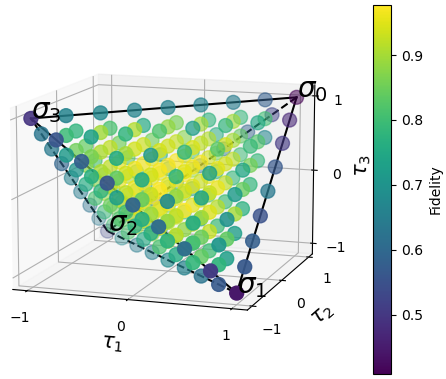
\includegraphics[width=0.45\textwidth]{fidelity-points.png}\\
\caption{Fidelities of one-qubit Pauli channels implemented on IBM's ibmq-lima.}
\label{fig: fidelity one qubit}
\end{figure}
\subsubsection{Pauli Dynamical Maps}
\label{subsec: Pauli Dynamical Maps}

A Pauli dynamical map is defined as a continuous parametrized 
curve drawn inside the set of Pauli channels and starting at the identity channel. 
Therefore, a Pauli dynamical map can be written as
\begin{eqnarray}
\mathcal{E}_p(\rho) = \sum_{\vec{\gamma}} k_{\vec{\gamma}}(p) \sigma_{\vec{\gamma}} \rho \sigma_{\vec{\gamma}},
\end{eqnarray}
where $p$ is a parameter in an interval $[a,b]$ 
and $\mathcal{E}_p$ is a Pauli channel for every $p$, 
with $\mathcal{E}_a$ being the identity channel.

Dynamical maps can be implemented using the same method as 
in figure \ref{fig: circuito}, with the only difference that now the state 
to be created on the ancilla qubits depends on parameter $p$ 
and therefore is given by 
\begin{equation}
\label{ec: parametrized state}
\sum_{\vec{\gamma}} b_{\vec{\gamma}}(p) |\vec{\gamma}\rangle
\end{equation}

\newpage